\documentclass[compress]{beamer}
\usepackage{ifthen,verbatim}

\newcommand{\isnote}{}
\xdefinecolor{lightyellow}{rgb}{1.,1.,0.25}
\xdefinecolor{darkblue}{rgb}{0.1,0.1,0.7}
\xdefinecolor{darkred}{rgb}{0.7,0.1,0.1}

%% Uncomment this to get annotations
%% \def\notes{\addtocounter{page}{-1}
%%            \renewcommand{\isnote}{*}
%% 	   \beamertemplateshadingbackground{lightyellow}{white}
%%            \begin{frame}
%%            \frametitle{Notes for the previous page (page \insertpagenumber)}
%%            \itemize}
%% \def\endnotes{\enditemize
%% 	      \end{frame}
%%               \beamertemplateshadingbackground{white}{white}
%%               \renewcommand{\isnote}{}}

%% Uncomment this to not get annotations
\def\notes{\comment}
\def\endnotes{\endcomment}

\setbeamertemplate{navigation symbols}{}
\setbeamertemplate{headline}{\mbox{ } \hfill
\begin{minipage}{5.5 cm}
\vspace{-0.75 cm} \small
\end{minipage} \hfill
\begin{minipage}{4.5 cm}
\vspace{-0.75 cm} \small
\begin{flushright}
\ifthenelse{\equal{\insertpagenumber}{1}}{}{Jim Pivarski \hspace{0.2 cm} \insertpagenumber\isnote/\pageref{numpages}}
\end{flushright}
\end{minipage}\mbox{\hspace{0.2 cm}}\includegraphics[height=1 cm]{../cmslogo} \hspace{0.1 cm} \includegraphics[height=1 cm]{../tamulogo} \hspace{0.01 cm} \vspace{-1.05 cm}}

\begin{document}
\begin{frame}
\vfill
\begin{center}
\textcolor{darkblue}{\Large Triggers for Muon Alignment}

\vfill
\begin{columns}
\column{0.3\linewidth}
\begin{center}
\large
\textcolor{darkblue}{Jim Pivarski}
\end{center}
\end{columns}

\begin{columns}
\column{0.3\linewidth}
\begin{center}
\scriptsize
{\it Texas A\&M University}
\end{center}
\end{columns}

\vfill
 4 February, 2009

\end{center}
\end{frame}

%% \begin{notes}
%% \item This is the annotated version of my talk.
%% \item If you want the version that I am presenting, download the one
%% labeled ``slides'' on Indico (or just ignore these yellow pages).
%% \item The annotated version is provided for extra detail and a written
%% record of comments that I intend to make orally.
%% \item Yellow notes refer to the content on the {\it previous} page.
%% \item All other slides are identical for the two versions.
%% \end{notes}

\small

\begin{frame}
\frametitle{Motivation}
\begin{itemize}
\item Track-based alignment measures relative positions of detectors through residuals on the tracks that connect them
\item Having ``enough'' tracks is a matter of connecting and completing the graph: samples are important for qualitatively different reasons
\item Relevant triggers: \only<1>{\it \scriptsize (next page)}\only<2-4>{single-muons, }\only<3-4>{\textcolor{darkblue}{beam-halo,} }\only<4>{\textcolor{darkred}{cosmic rays}}
\end{itemize}

\begin{center}
\only<1>{\includegraphics[width=0.8\linewidth]{graph_pointsonly.png}}
\only<2>{\includegraphics[width=0.8\linewidth]{graph_collisions.png}}
\only<3>{\includegraphics[width=0.8\linewidth]{graph_beamhalo.png}}
\only<4>{\includegraphics[width=0.8\linewidth]{graph_cosmics.png}}
\end{center}
%% \hspace{-0.83 cm} \textcolor{darkblue}{\Large Outline2}
\end{frame}

%% \section*{First section}
%% \begin{frame}
%% \begin{center}
%% \Huge \textcolor{blue}{First section}
%% \end{center}
%% \end{frame}

\begin{frame}
\frametitle{Outline for this talk}
\begin{itemize}\setlength{\itemsep}{0.5 cm}
\item Why the existing single-muon triggers are sufficient
\item Why the tracker-pointing cosmics trigger will be sufficient
\item CSC beam-halo trigger

\vspace{0.1 cm}
\begin{itemize}\setlength{\itemsep}{0.25 cm}
\item radial distribution, special ``CSC overlaps'' events
\item calculation of required rate from alignment resolution
\item implementation, monitoring, people/institutions
\end{itemize}
\end{itemize}
\end{frame}

\begin{frame}
\frametitle{Single-muon triggers}

\vspace{-0.3 cm}
\begin{columns}
\column{0.7\linewidth}

\begin{itemize}
\item Objective is to find the peak of the residuals distribution
  of each muon chamber with a resolution of 200--300~$\mu$m \mbox{about once a month\hspace{-1 cm}}
\item Distribution is broadened by propagation uncertainty
  (core) and muon scattering (tails)
\item Scattering tails are highly dependent on \mbox{track $p_T$\hspace{-1 cm}} \\ (top plot
  from CRAFT, note log scale)
\item Cutting low on $p_T$\ldots

\vspace{-0.2 cm}
\begin{itemize}
\item increases statistics, which helps
\item adds tails, which hurts
\end{itemize}
\vspace{-0.2 cm}

\item Optimum is $p_T \gtrsim$ 10~GeV

\vspace{-0.2 cm}
\begin{itemize}
\item tested different $p_T$ cuts in CSA08 with inclusive single muons (bottom plot)
\item figure of merit is statistics-only; systematics better controlled at high $p_T$
\end{itemize}
\vspace{-0.2 cm}

\item 8E29 and 1E31 muon triggers are unprescaled above 9~GeV \textcolor{red}{$\surd$}
\end{itemize}

\column{0.3\linewidth}

\vspace{0.75 cm}
\includegraphics[width=\linewidth]{residuals_barrel.pdf}

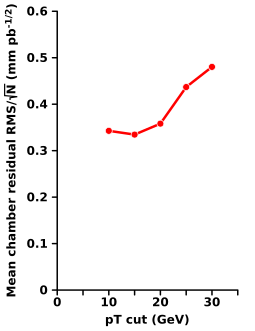
\includegraphics[width=\linewidth]{collisions_resolution.png}
\end{columns}
\end{frame}

\begin{frame}
\frametitle{Tracker-pointing cosmic rays}

\begin{itemize}
\item Collisions muons in a given chamber all pass through the same part of the tracker: a major source of systematic error
\item Cosmic rays make the graph of alignables more complete, allowing us to diagnose muon alignment as a function of track source

\hfill \mbox{\includegraphics[height=3.2 cm]{tracker_xray.png} \hspace{0.3 cm} \includegraphics[height=3.2 cm]{zresid_from_tracker_outerbottom.png}} \hfill
\end{itemize}

\vspace{0.2 cm}
\hspace{-0.83 cm} \textcolor{darkblue}{\Large What cosmic rays do we need?}

\begin{itemize}
\item Exactly the same cosmic rays the tracker alignment needs
\item ``All of them'' = $\mathcal{O}(\mbox{few Hz})$ (between bunch crossings)
\item If rate-limited, apply a $\phi$-dependent prescale (see Andrei's talk)
\end{itemize}
\end{frame}

\begin{frame}
\frametitle{Beam-halo in the muon endcaps}

\begin{itemize}\setlength{\itemsep}{0.2 cm}
\item Useful for early and rapid CSC alignment
\begin{itemize}\setlength{\itemsep}{0.2 cm}
\item track-based alignment of ME$-$2/1, ME$-$3/1 demonstrated \mbox{with\hspace{-1 cm}} \\ 270~$\mu$m accuracy in the September 2008 run

{\scriptsize validation of track-based alignment against an independent method:}

\mbox{\hspace{-1 cm}\includegraphics[width=3.8 cm, angle=90]{compare_m31_x.pdf} \includegraphics[height=3.8 cm]{delta_translations.pdf}}

\item takes advantage of physical overlap of pairs of chambers to compare tracks with very small propagation uncertainties

\item an important part of the design of the muon endcap

\end{itemize}

\item Beam-halo events are also useful for general CSC detector studies
\end{itemize}
\end{frame}

\begin{frame}
\frametitle{What is our signal rate?}
\begin{itemize}\setlength{\itemsep}{0.25 cm}
\item \textcolor{darkblue}{Unknown:} Monte Carlo differs from data, which differs from data

\vspace{0.1 cm}
\mbox{\hspace{-1 cm} \includegraphics[height=0.33\linewidth]{beam-halo.png} \includegraphics[height=0.33\linewidth]{spot_62084.png} \includegraphics[height=0.33\linewidth]{spot_62096.png}}

\vspace{0.1 cm}
\item LHC beam-halo will at some point ``settle down'' into a steady state, but we can't know the exact profile yet

\item We do know that the CSC inner ring (ring 1) will get more muons than the CSC outer ring (ring 2)

\item There are twice as many chambers in ring 2 as ring 1; \\ we'd like to balance the load
\end{itemize}
\end{frame}

\begin{frame}
\frametitle{CSC beam-halo HLT paths}

\begin{columns}
\column{0.8\linewidth}

\begin{itemize}
\item \textcolor{darkblue}{HLT\_CSCBeamHalo} only passes the L1 bit (\textcolor{darkblue}{L1\_SingleMuBeamHalo}): can be prescaled if \mbox{necessary\hspace{-1 cm}}
\item \textcolor{darkblue}{HLT\_CSCBeamHaloRing2or3:} for general studies of outer detectors, less prescaled
\item \textcolor{darkblue}{HLT\_CSCBeamHaloOverlapsRing1, Ring2:} \\ special events for alignment where track passes through pair of neighboring chambers \\ \mbox{\scriptsize (rate is about 1/50$^{\mbox{\scriptsize th}}$ of general beam-halo due to geometry)}
\end{itemize}

\column{0.2\linewidth}

\includegraphics[width=\linewidth]{overlaps.png}
\end{columns}

\begin{center}
\includegraphics[width=0.85\linewidth]{venn_diagram.png}
\end{center}
\end{frame}

\begin{frame}
\frametitle{Implementation details}

\begin{itemize}
\item Level 1: standard CSC trigger with a non-interaction point $|\eta|$ \mbox{window\hspace{-1 cm}} \\ (in the global menu, not a technical trigger)

\item HLT: identifies ring with a minimum number of hltCsc2DRecHits

\item identifies ``overlap'' by proximity of hits in neighboring chambers \\ (no tracking)
\end{itemize}

\vfill
\hspace{-0.83 cm} \textcolor{darkblue}{\Large What are our rate requirements?}

\begin{itemize}
\item 2008 alignment used 33,000 {\scriptsize HLT\_CSCBeamHaloOverlapsRing1} events

\vspace{0.1 cm}
\begin{columns}
\column{0.7\linewidth}

\renewcommand{\arraystretch}{1.2} \begin{tabular}{c c}
& 1 alignment/day \mbox{\scriptsize (a comfortable redundancy)\hspace{-3.5 cm}} \\
{\scriptsize HLT\_CSCBeamHaloOverlapsRing1} & 0.4~Hz \\
{\scriptsize HLT\_CSCBeamHaloOverlapsRing2} & 0.8~Hz \\
{\scriptsize HLT\_CSCBeamHalo} & $\mathcal{O}(\mbox{0.1--1~Hz})$ \\
{\scriptsize HLT\_CSCBeamHaloRing2or3} & 2$\times$ the above \\
\end{tabular}

\column{0.4\linewidth}

\vspace{0.7 cm}
\includegraphics[width=1.05\linewidth]{overlaps_straight_through.png}

\vspace{-0.7 cm}
\vspace{-\baselineskip}
\mbox{ }
\end{columns}

\vspace{0.1 cm}
\item Overlaps are strictly necessary for alignment; \\ other beam-halo events are used in cross-checks
\end{itemize}
\end{frame}

\begin{frame}
\frametitle{Monitoring/Ownership}

\begin{columns}
\column{0.6\linewidth}
\begin{itemize}
\item Maintainance of CSC beam-halo triggers (L1 and HLT): \\ \textcolor{darkblue}{Joseph Gartner, U.\ Florida}
\item Developed L1 beam-halo trigger diagnostics and monitoring \\ L1 $\to$ HLT full-chain efficiency
\end{itemize}

\vspace{0.65 cm}

\column{0.4\linewidth}
\includegraphics[width=\linewidth]{TriggerOcc.png}

\textcolor{blue}{\mbox{\hspace{-1.4 cm}} \tt \tiny \href{http://tier2.ihepa.ufl.edu/~gartner/plots/Cosmics/}{http://tier2.ihepa.ufl.edu/$\sim$gartner/plots/Cosmics/}\mbox{\hspace{-2 cm}}}
\end{columns}

\vspace{-0.65 cm}
\begin{columns}
\column{1.06\linewidth}
\textcolor{darkblue}{Future plans:}
\begin{itemize}
\item Monitor more continuous distributions (e.g.\ radius, $\phi$ of hits)
\item More HLT-level diagnostics
\item Regular release validation for the 3\_0\_X cycle
\begin{itemize}
\item DQM module already exists in {\tt \tiny HLTriggerOffline/special/src/HaloTrigger.cc}
\end{itemize}

\end{itemize}
\end{columns}

\vspace{0.5 cm}
\hspace{-0.83 cm} \textcolor{darkblue}{\Large Answers to other questions:}

\vspace{0.2 cm}
\textcolor{darkblue}{Primary dataset?} can be the same as cosmic ray sample, but not \mbox{collisions\hspace{-1 cm}}

\vspace{0.2 cm}
\textcolor{darkblue}{Range of luminosities?} at least through the 1$\times$10$^{31}$ era
\end{frame}

\begin{frame}
\frametitle{Summary}
\begin{itemize}\setlength{\itemsep}{0.25 cm}
\item Primary alignment workflows rely on single-muon triggers, but
  offline $p_T > 10$~GeV requirement makes proposed 8E29 and 1E31
  menus (and any conceivable variant) acceptable

\item Cosmic rays are needed to resolve systematic uncertainties, but
  we need tracker-pointing cosmics, just like tracker alignment group
\begin{itemize}\setlength{\itemsep}{0.1 cm}
\item ``all'' of the tracker-pointing cosmics (a few Hz) would be \mbox{useful\hspace{-1 cm}}
\item see Andrei's talk for details
\end{itemize}

\item Beam-halo can align the muon endcaps early and on short \mbox{timescales\hspace{-1 cm}}
\begin{itemize}\setlength{\itemsep}{0.1 cm}
\item demonstration of high accuracy with real beam in 2008
\item existing triggers can adjust for as-yet unknown radial \mbox{distribution\hspace{-1 cm}}
\item 1 alignment/day requires 2--4~Hz
\item responsible person/institution: Joseph Gartner, U.\ Florida
\end{itemize}

\item One last note: muon hardware alignment data are {\it not}
  transferred through the abort gap--- no trigger issues

\end{itemize}
\label{numpages}
\end{frame}

\end{document}
